%----------------------------------------------------------------------------
\chapter{A Poisson egyenlet diszkretizálása és megoldási módszerei}
%----------------------------------------------------------------------------
Ha feltételezhető az egyenlet megoldásáról, hogy "elég" sima, akkor a függvény egy adott pont környékén jól közelíthető az érintőjével.
Más szavakkal: a parciális deriváltak Taylor sorának első eleme domináns és a többi elhanyagolásával csupán kis hibát vétünk.
Ezt a gondolatot felhasználva jutunk el a véges differenciák módszeréhez, ami a következő lépésekből áll:
\begin{itemize}
\item a tartományra háló illesztése: jelen esetben ekvidisztáns pontháló
\item a deriváltak közelítése érintő meredekségével
\item az előző lépéssel adódó algebrai egyenletének felírása
\item ennek az egyenletnek a megoldása
\end{itemize}
Nagy hangsúlyt kell fektetni a feltételezés realitásának a vizsgálatába, mivel könnyen lehetséges, hogy a módszer által kiadódó megoldás nem az eredeti probléma megoldásához konvergál (vagy divergál).

\section{A probléma definiálása}
A Laplace egyenlet megoldását a követekező 2D-s tartományon keresem:
\begin{figure}[!ht]
\centering
%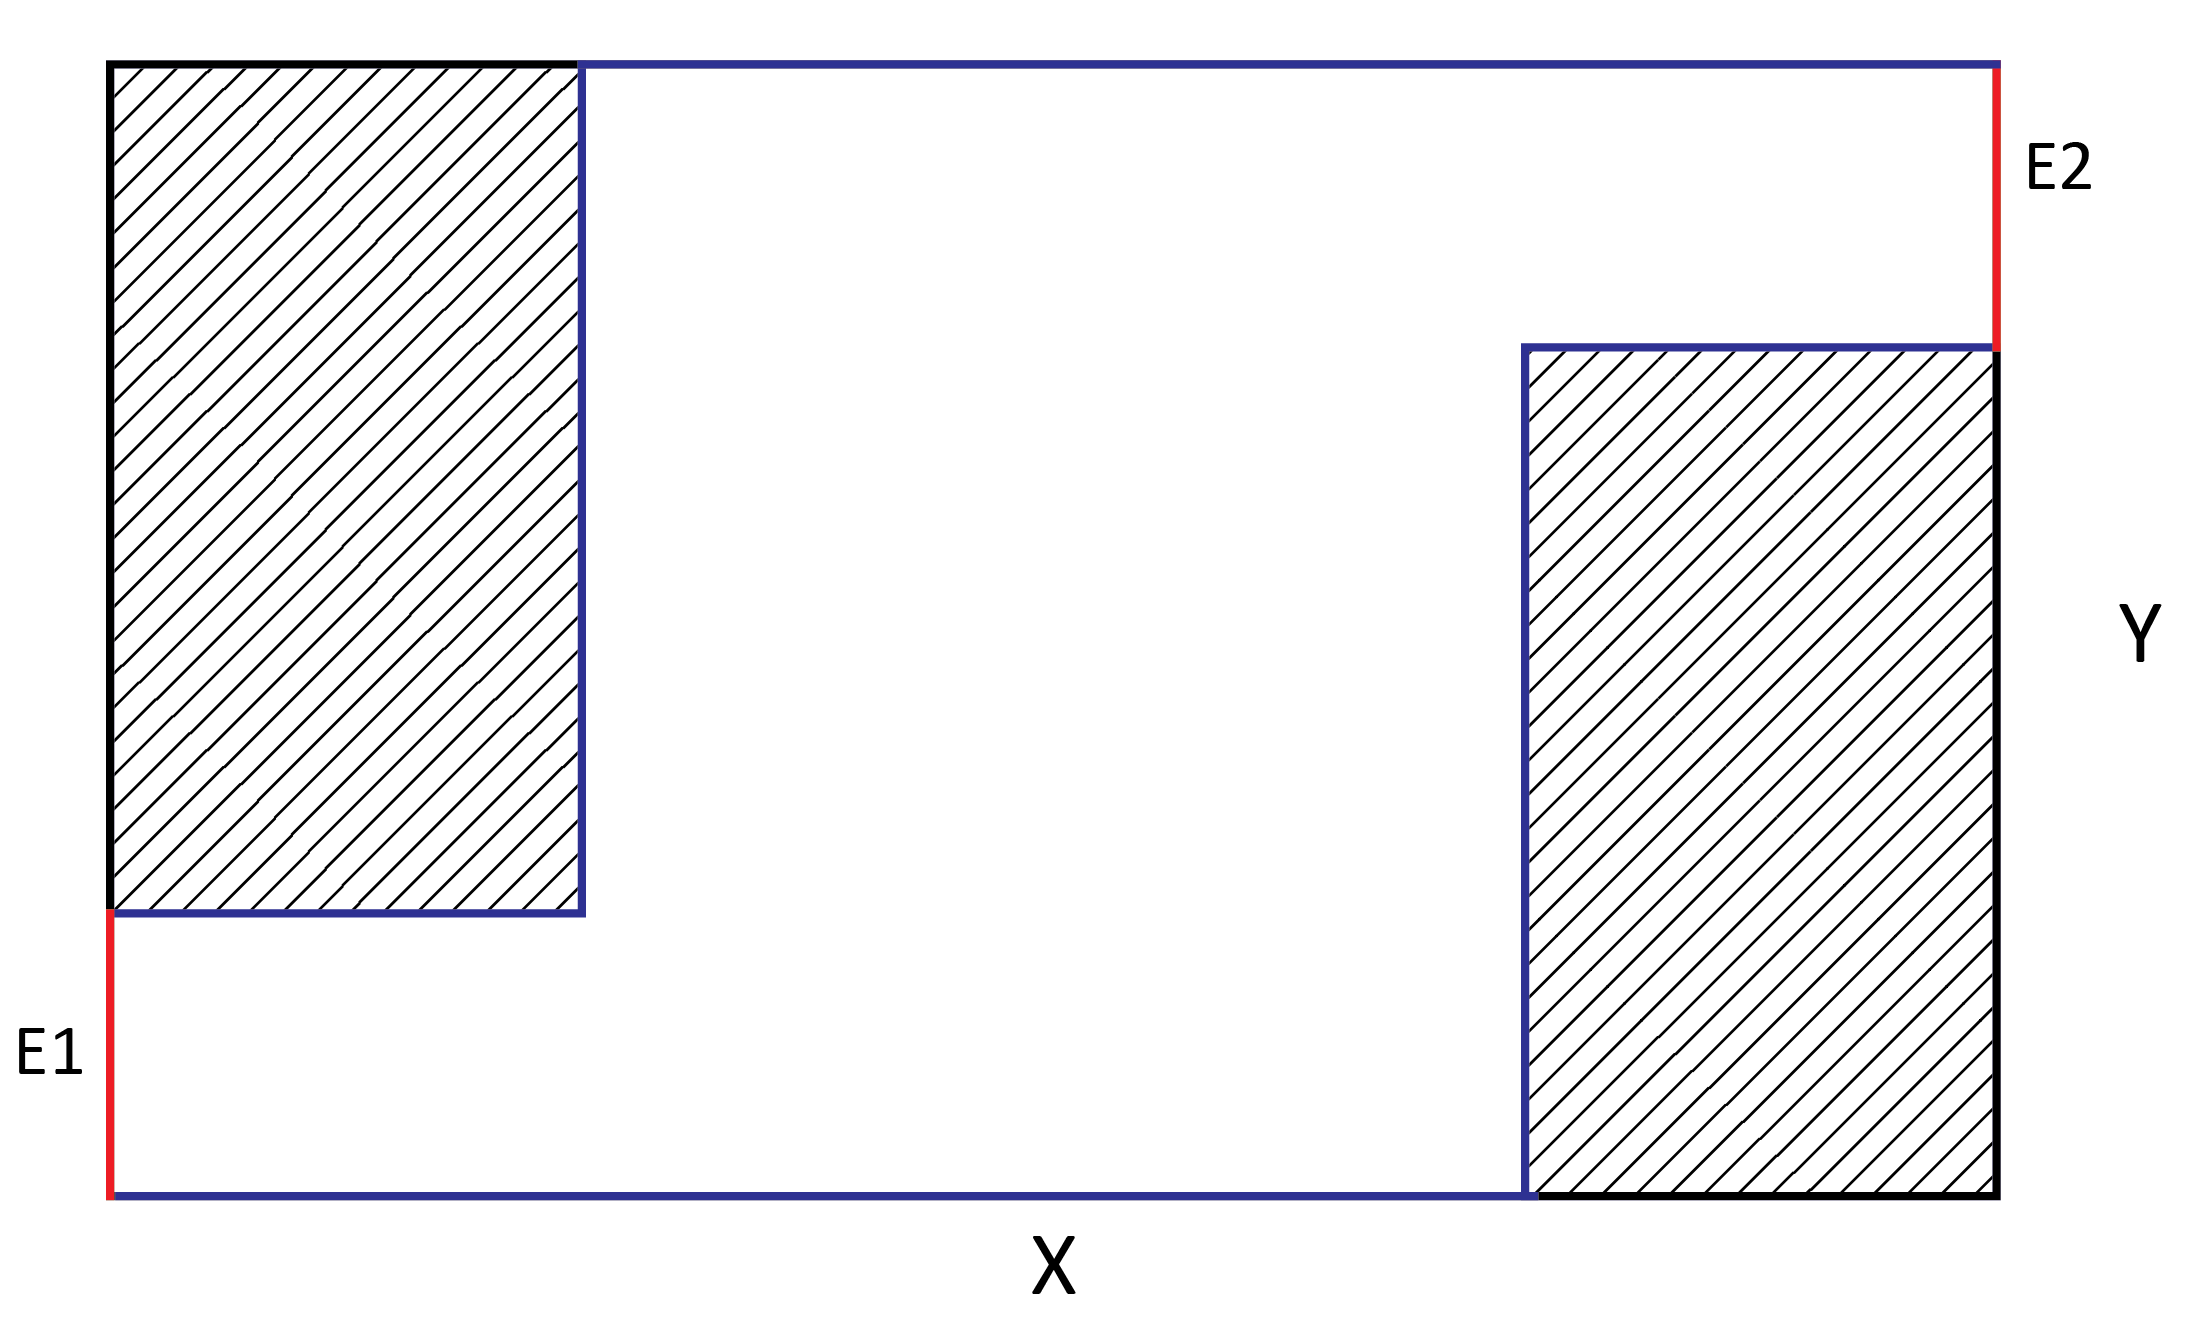
\includegraphics[width=150mm, keepaspectratio]{figures/domain.png}
\caption{A megoldandó tartomány} 
%\label{fig:equivTV}
\end{figure}
A problémához tartozó peremfeltétel a következőképp definiálódik:
\begin{itemize}
\item $E_1$ elektródán $\varphi_0 = 0 V$ potenciálú Dirichlet (piros) feltétel, 
\item $E_2$ elektróda $\varphi_1 = 1 V$ potenciálú Dirichlet (piros) feltétel,
\item mindenütt máshol homogén Neumann (kék) peremfeltétel érvényesül.
\end{itemize}
Az objektum $x$ irányú kiterjedése $X = 500$, $y$ irányú kiterjedése $Y=500$ értékű. Az osztópontok az oldalél $\tfrac14$ és $\tfrac34$-nél található.


%----------------------------------------------------------------------------
\section{A háló illesztése}
%----------------------------------------------------------------------------
A háló az adott geometriát egyenletesen elosztott pontokkal fedi le.
A tartományt $x$ és $y$ irányban is $N$ pontra bontottam fel.
Adott pont megkülönböztetésére létrehoztam egy mátrixot, ami azonos méretű mint a háló.
A mátrix egy adott értéke megadja, hogy azzal a ponttal milyen egyenlet írandó fel.
\begin{figure}[H]
\centering
%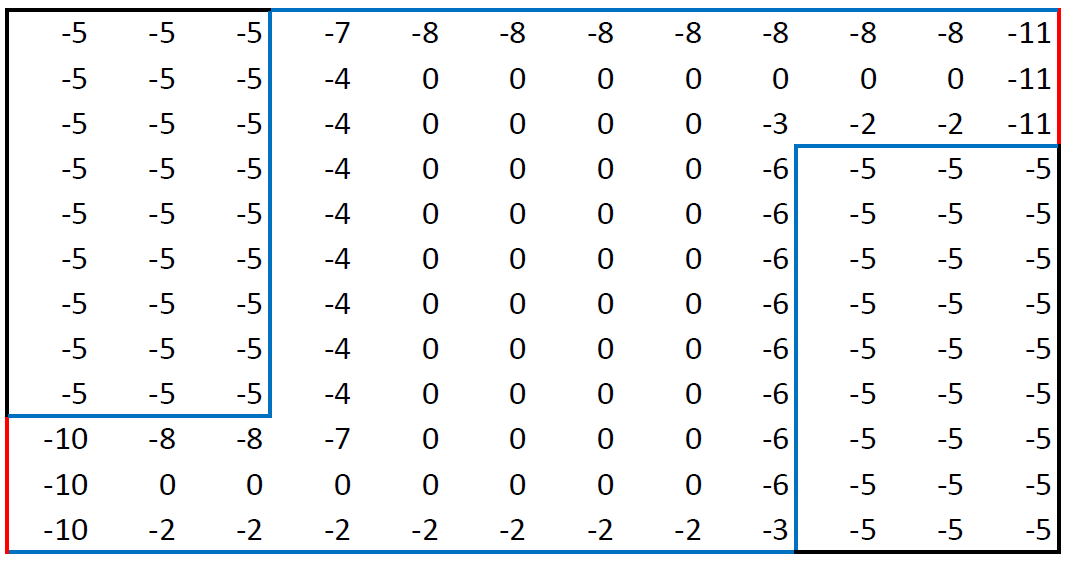
\includegraphics[width=150mm, keepaspectratio]{figures/pvals.png}
\caption{A háló pontjaihoz tartozó mátrix} 
%\label{fig:equivTV}
\end{figure}
\begin{table}
\centering
\begin{tabular}{|r|rc|}
\hline
érték & \multicolumn{2}{r|}{egyenlet}\\
\hline\hline
-5 & \multicolumn{2}{r|}{nem tartozik hozzá egyenlet}\\
0 & \multicolumn{2}{r|}{általános differencia egyenlet}\\
\hline
-4 & homogén Neumann & balra\\
-8 & homogén Neumann & fel\\
-6 & homogén Neumann & jobbra\\
-2 & homogén Neumann & le\\
-7 & homogén Neumann & balra-fel\\
-9 & homogén Neumann & jobbra-fel\\
-3 & homogén Neumann & jobbra-le\\
-1 & homogén Neumann & balra-le\\
\hline
-10 & \multicolumn{2}{r|}{$\varphi_0$ értékű Dirichlet feltétel}\\
-11 & \multicolumn{2}{r|}{$\varphi_1$ értékű Dirichlet feltétel}\\
\hline
\end{tabular}
\caption{A háló pontjaihoz tartozó mátrix értékeinek magyarázata} 
\end{table}

%----------------------------------------------------------------------------
\section{Deriváltak közelítése és az egyenlet megoldása}
%----------------------------------------------------------------------------
A diszkretizálás során használt jelölést a következő ábra tartalmazza:
\begin{figure}[H]
\centering
%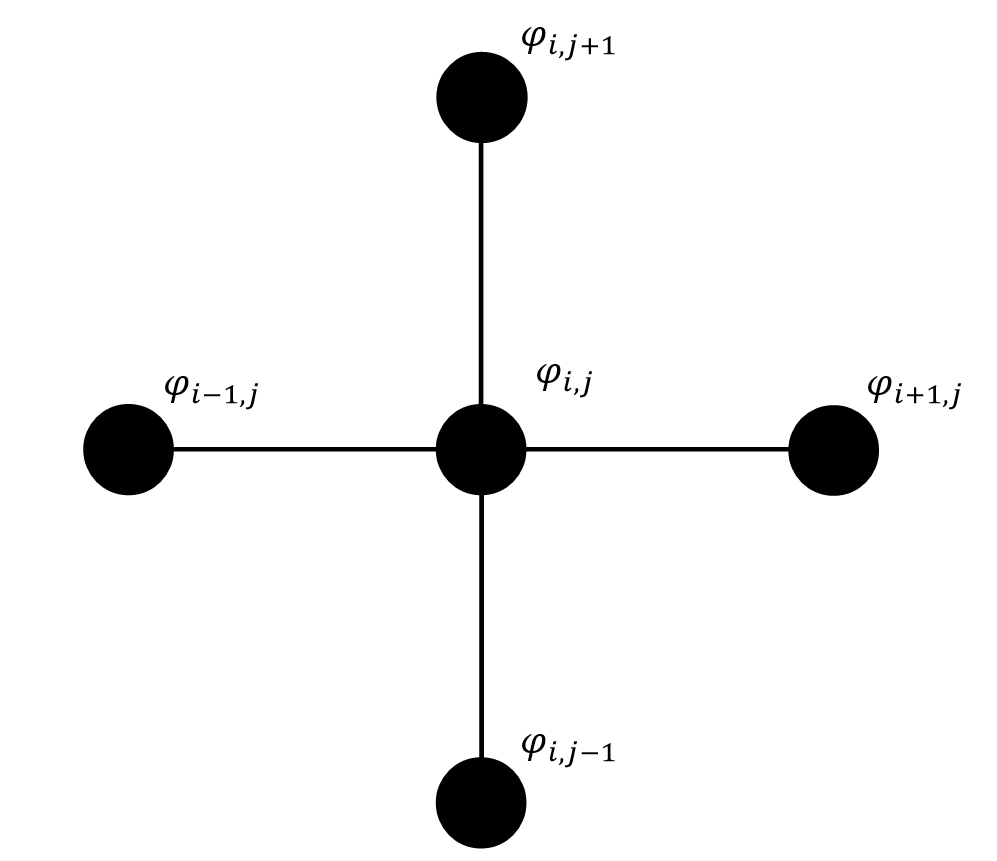
\includegraphics[width=80mm, keepaspectratio]{figures/points.png}
\caption{Az 5-pontos séma során használt jelölés} 
%\label{fig:equivTV}
\end{figure}
A Poisson egyenlet baloldalán található kétszeres deriváltat a következőképp közelíthetjük az általános 5-pontos sémával:
\begin{align}
\left.\nabla^2 \varphi\right|_{i,j} = \left(\cfrac{\partial^2}{\partial x^2}+\cfrac{\partial^2}{\partial y^2}\right) \varphi_{i,j} &\approx
\cfrac{\varphi_{i+1,j}-2\varphi_{i,j}+\varphi_{i-1,j}}{h^2} +
\cfrac{\varphi_{i,j+1}-2\varphi_{i,j}+\varphi_{i,j-1}}{h^2} =\\
\left.\nabla^2\right|_{i,j} &\approx
\cfrac{\varphi_{i+1,j}+\varphi_{i,j+1}-4\varphi_{i,j}+\varphi_{i-1,j}+\varphi_{i,j-1}}{h^2}
\end{align}
Ezt a Poisson egyenletbe behelyettesítve
\begin{align}
\cfrac{\varphi_{i+1,j}+\varphi_{i,j+1}-4\varphi_{i,j}+\varphi_{i-1,j}+\varphi_{i,j-1}}{h^2} = f(i,j)
\end{align}
Ezt mátrixok alakba öltve a szokásos egyenletrendszer $\mathbf{A}\Phi = F$ alakját veszi fel.
Mivel az eggyüthatómátrix tridiagonális blokkmátrix, így relatíve könnyen meg lehet oldani.

A dolgozatom során - később ismertetett indokok miatt - az iteratív megoldást használom.
Egy adott $(i,j)$ ponthoz tartozó potenciál értékét ki lehet fejezni az alábbiképp:
\begin{equation}
\varphi_{i,j} = \cfrac{-h^2\cdot f(i,j) +\varphi_{i+1,j}+\varphi_{i,j+1}+\varphi_{i-1,j}+\varphi_{i,j-1}}{4}
\end{equation}
Ha nincs beiktatott töltés, akkor ez épp az adott pont szomszédjainak az átlaga. 
A potenciálok értékét iteratíve frissítve ezzel a kifejezéssel
konvergálni fog a megoldáshoz.
Adott pont aktuális potenciáljának értéke a szomszédos potenciálok
korábbi értékéből számítódik.
E számítás szintén el lehet gyorsan végezni és nagy előnye, hogy kevesebb memóriát fogyaszt.

